% Векторизация операций над матрицами малой размерности.
\subsection{Векторизация операций над матрицами малой размерности для процессора \\ Intel Xeon Phi Knights Landing}

\subsubsection{Умножение матрицы $8 \times 8$ на вектор}

Реализация неоптимизированной версии может выглядеть следующим образом:

\begin{lstlisting}[caption={Невекторизованная версия умножения матрицы размера $8 \times 8$ на вектор},label={lst:text_4_small_matr_8x8_mul_vel_noopt}]
void matvec8_orig(float* __restrict m,
                  float* __restrict v,
                  float* __restrict r)
{
    for (int i = 0; i < V8; i++)
    {
        float sum = 0.0;
        int ii = i * V8;

        for (int j = 0; j < V8; j++)
        {
            sum = sum + m[ii + j] * v[j];
        }

        r[i] = sum;
     }
}
\end{lstlisting}

Рассмотрим некоторые моменты реализации.
Матрица хранится в сплошной области памяти по строкам и передается в фунцию через указатель на начало этой области.
Все параметры функции передаются c указанием \texttt{\_\_restrict} для облегчения компилятору задачи по оптимизации.
Умножение матрицы на вектор состоит в вычислении скалярного произведения каждой строки этой матрицы на вектор и составлении из результатов выходного вектора.
Так как в данном случае размер строки матрицы равен 8 элементам типа float, то одной операцией в 512-битный регистр можно загрузить из памяти сразу 2 соседние строки матрицы.
После чего нужно выполнить операцию упакованного умножения на регистр, содержащий две копии вектора, на который умножается матрица (выполнить запись двух копий вектора в zmm регистр можно с помощью операции gather).
Сумма первых восьми элементов получившегося регистра и последних восьми элементов будут являться элементами выходного вектора r (см. рис. 1).

\begin{figure}[ht]
	\centering
		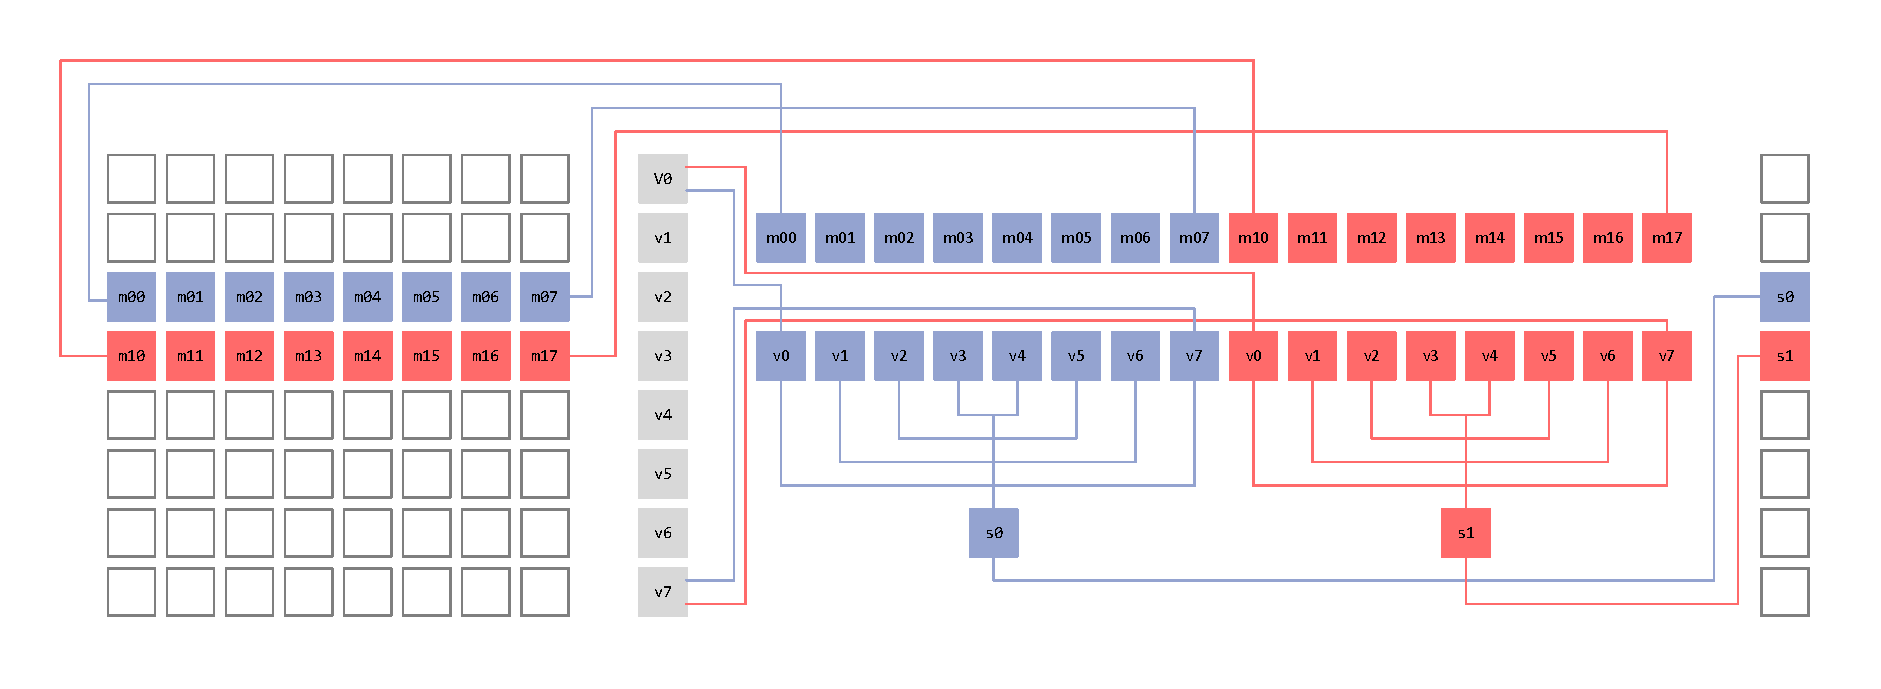
\includegraphics[width=1.00\textwidth]{./pics/text_4_small_matr/matvec8.pdf}
	\caption{Схема вычисления результата в операции matvec8}
	\label{fig:text_4_small_matr_matvec8}
\end{figure}

Итак, при реализации операции умножения матрицы 8x8 на вектор мы должны загрузить всю матрицу в четыре zmm регистра.
Затем выполнить четыре упакованные операции умножения этих регистров, на регистр, содержащий две копии вектора, на которые умножается матрица.
После этого из каждого из получившихся четырех регистров мы должны получить сумму элементов каждой его половины, что в результате даст 8 искомых элементов выходного вектора.
Получение суммы элементов половины zmm регистра представляет собой как раз ту горизонтальную операцию, реализация которой в помощью интринсика оказывается слишком дорогой.
Как показали эксперименты, простое применение интринсика \texttt{\_mm512\_mask\_reduce\_add\_ps} (и даже безмасочного \texttt{\_mm512\_reduce\_add\_ps} в случае умножения матрицы 16x16) не приводит к ускорению по сравнению с оригинальной версией функции, оптимизированной компилятором icc с использованием уровня оптимизации -O3.
Прежде чем переходить к оптимизации данных горизонтальных операций рассмотрим второй интересующий нас пример, -- перемножение двух матриц размера 8x8, -- и убедимся, что в этом случае проявляется та же проблема.

\subsubsection{Перемножение матриц размера $8 \times 8$}

Как и в случае с первым примером, вначале приведем простую реализацию неоптимизированной версии перемножения двух матриц размера 8x8:

\begin{lstlisting}[caption={Невекторизованная версия перемножения матриц размера $8 \times 8$}, label={lst:text_4_small_matr_8x8_mul_matr_noopt}]
void matmat8_orig(float* __restrict a,
                  float* __restrict b,
                  float* __restrict r)
{
    for (int i = 0; i < V8; i++)
    {
        int ii = i * V8;
 
        for (int j = 0; j < V8; j++)
        {
            float sum = 0.0;

            for (int k = 0; k < V8; k++)
            {
                int kk = k * V8;
                
                sum = sum + a[ii + k] * b[kk + j];
            }

            r[ii + j] = sum;
        }
    }
}
\end{lstlisting}

Логика перемножения двух матриц состоит в том, что результаты попарного скалярного произведения 8 строк матрицы $a$ и 8 столбцов матрицы $b$ формируют элементы результирующей матрицы.
Как и в предыдущем примере, использование 512-битных команд загрузки данных из памяти позволяет за одну операцию загрузить две соседние строки матрицы $a$ (операцией последовательного чтения) или два соседних столбца матрицы $b$ (с помощью операции gather).
После этого мы должны вычислить четыре скалярные произведения каждой половины загруженного из матрицы $a$ вектора с каждой половиной загруженного из матрицы $b$ вектора.
Для этого выполняются две операции поэлементного перемножения двух загруженных векторов, в одном из которых старшая и младшая половины второго вектора переставлены местами, как показано на рис. 2.

\begin{figure}[ht]
	\centering
		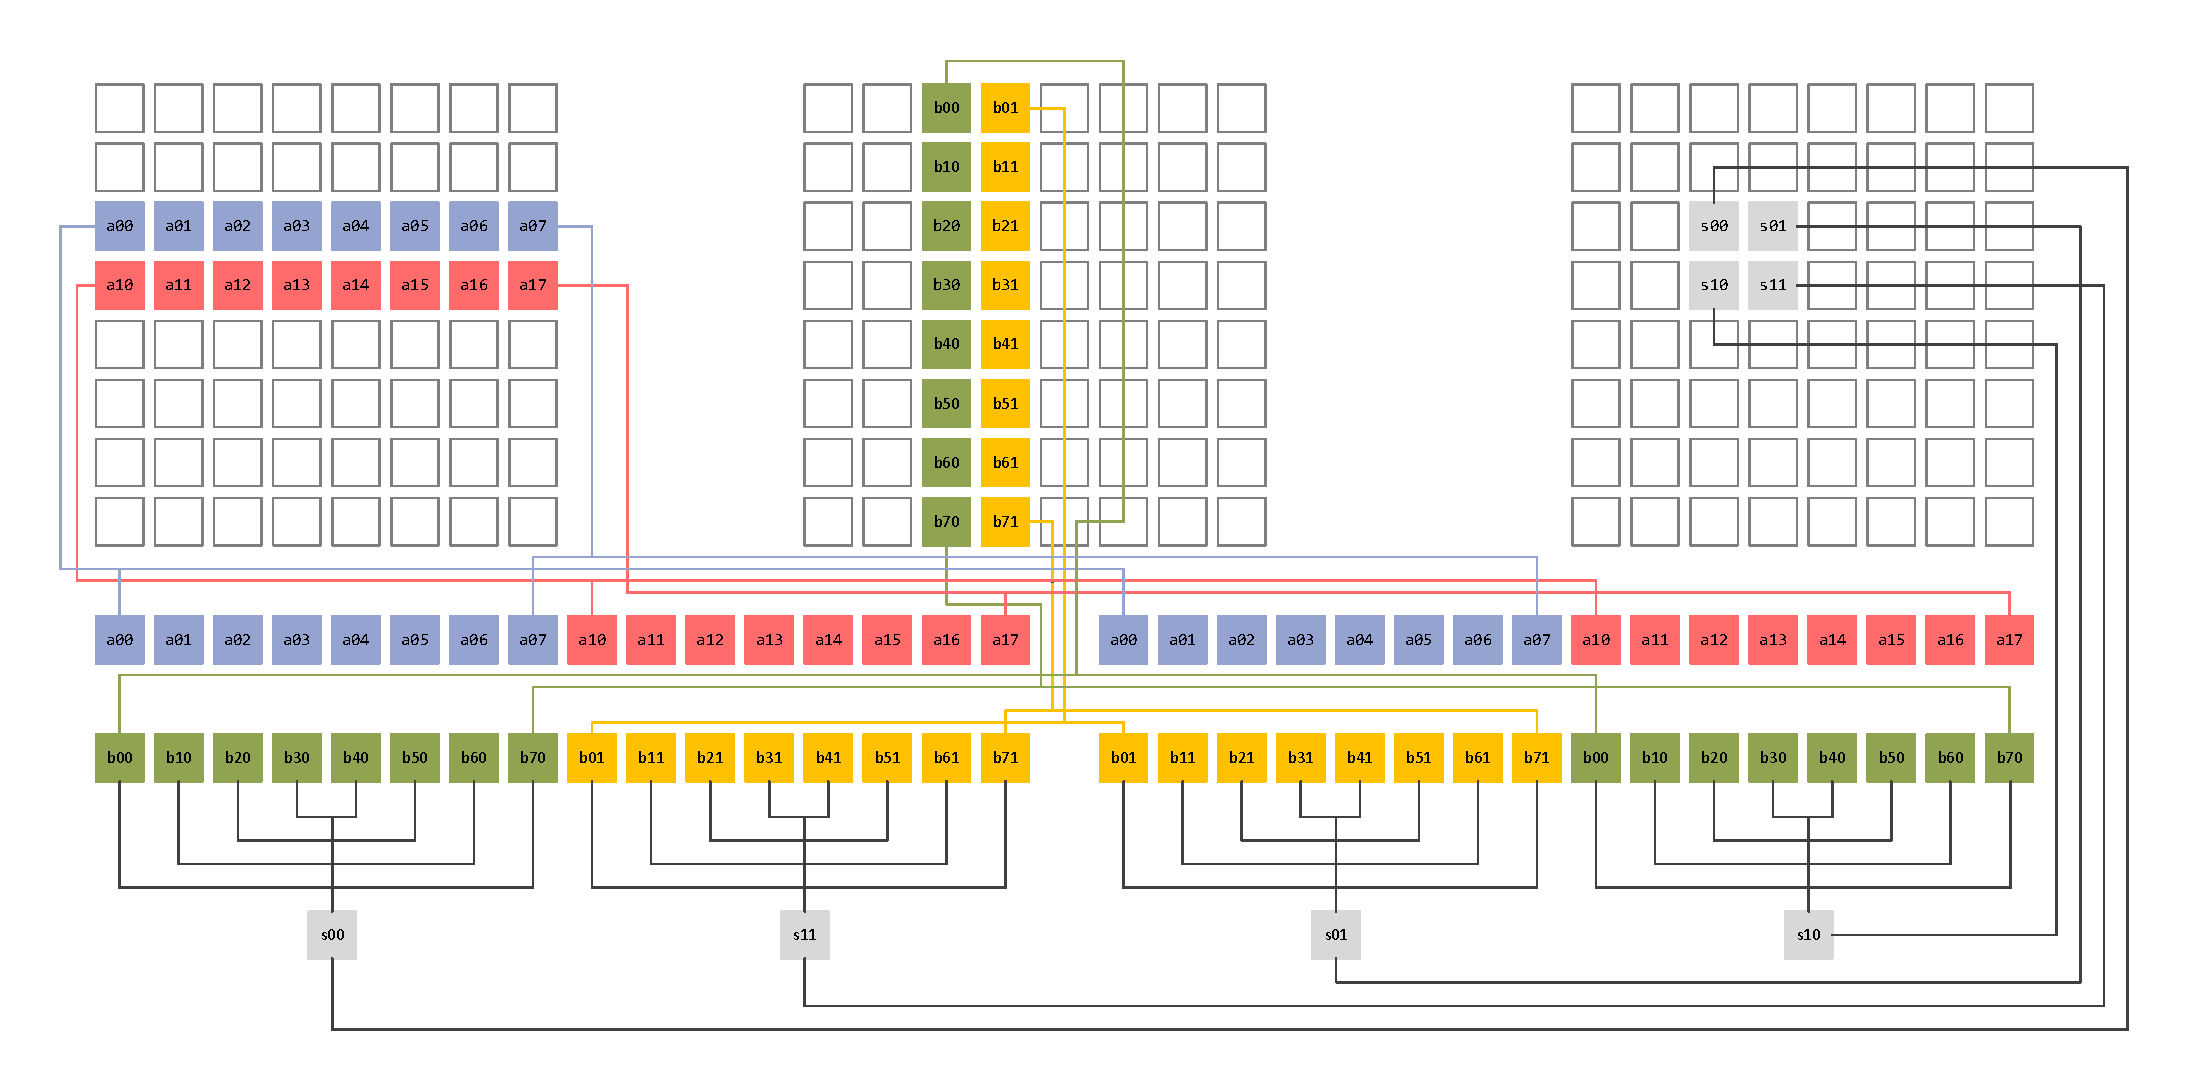
\includegraphics[width=1.00\textwidth]{./pics/text_4_small_matr/matmat8.pdf}
	\caption{Схема вычисления результата в операции matmat8}
	\label{fig:text_4_small_matr_matmat8}
\end{figure}

После выполнения данных действий снова возникает потребность вычисления суммы 8 младших элементов данного вектора и 8 старших элементов этого же вектора.
Таким образом, мы приходим к тому, что каждый элемент результирующей матрицы должен быть получен с помощью горизонтальной операции суммирования 8 младших или старших элементов некоторого zmm регистра.

Примеры реализаций функций \texttt{matvec16\_orig} и \texttt{matmat16\_orig} аналогичны, но там возникают задачи суммирования всех 16 элементов вектора.
Отсюда возникает потребность объединения таких горизонтальных операций вместе.
Рассмотрим задачу в общем виде: даны 16 zmm регистров (a, b, c, d, e, f, g, h, i, j, k, l, m, n, o, p), каждый из которых содержит по 16 элементов типа float.
Требуется посчитать суммы их элементов и записать в один регистр zmm.
Набор команд AVX-512 и библиотека интринсиков содержат все необходимые возможности для эффективной реализации данного функционала.
Схема вычислений состоит из четырех фаз, каждая из которых реализуется операциями перестановок с последующим сложением и слиянием векторов.
На рис. 3 представлена схема суммирования элементов для пары векторов (a и b).

\begin{figure}[ht]
	\centering
		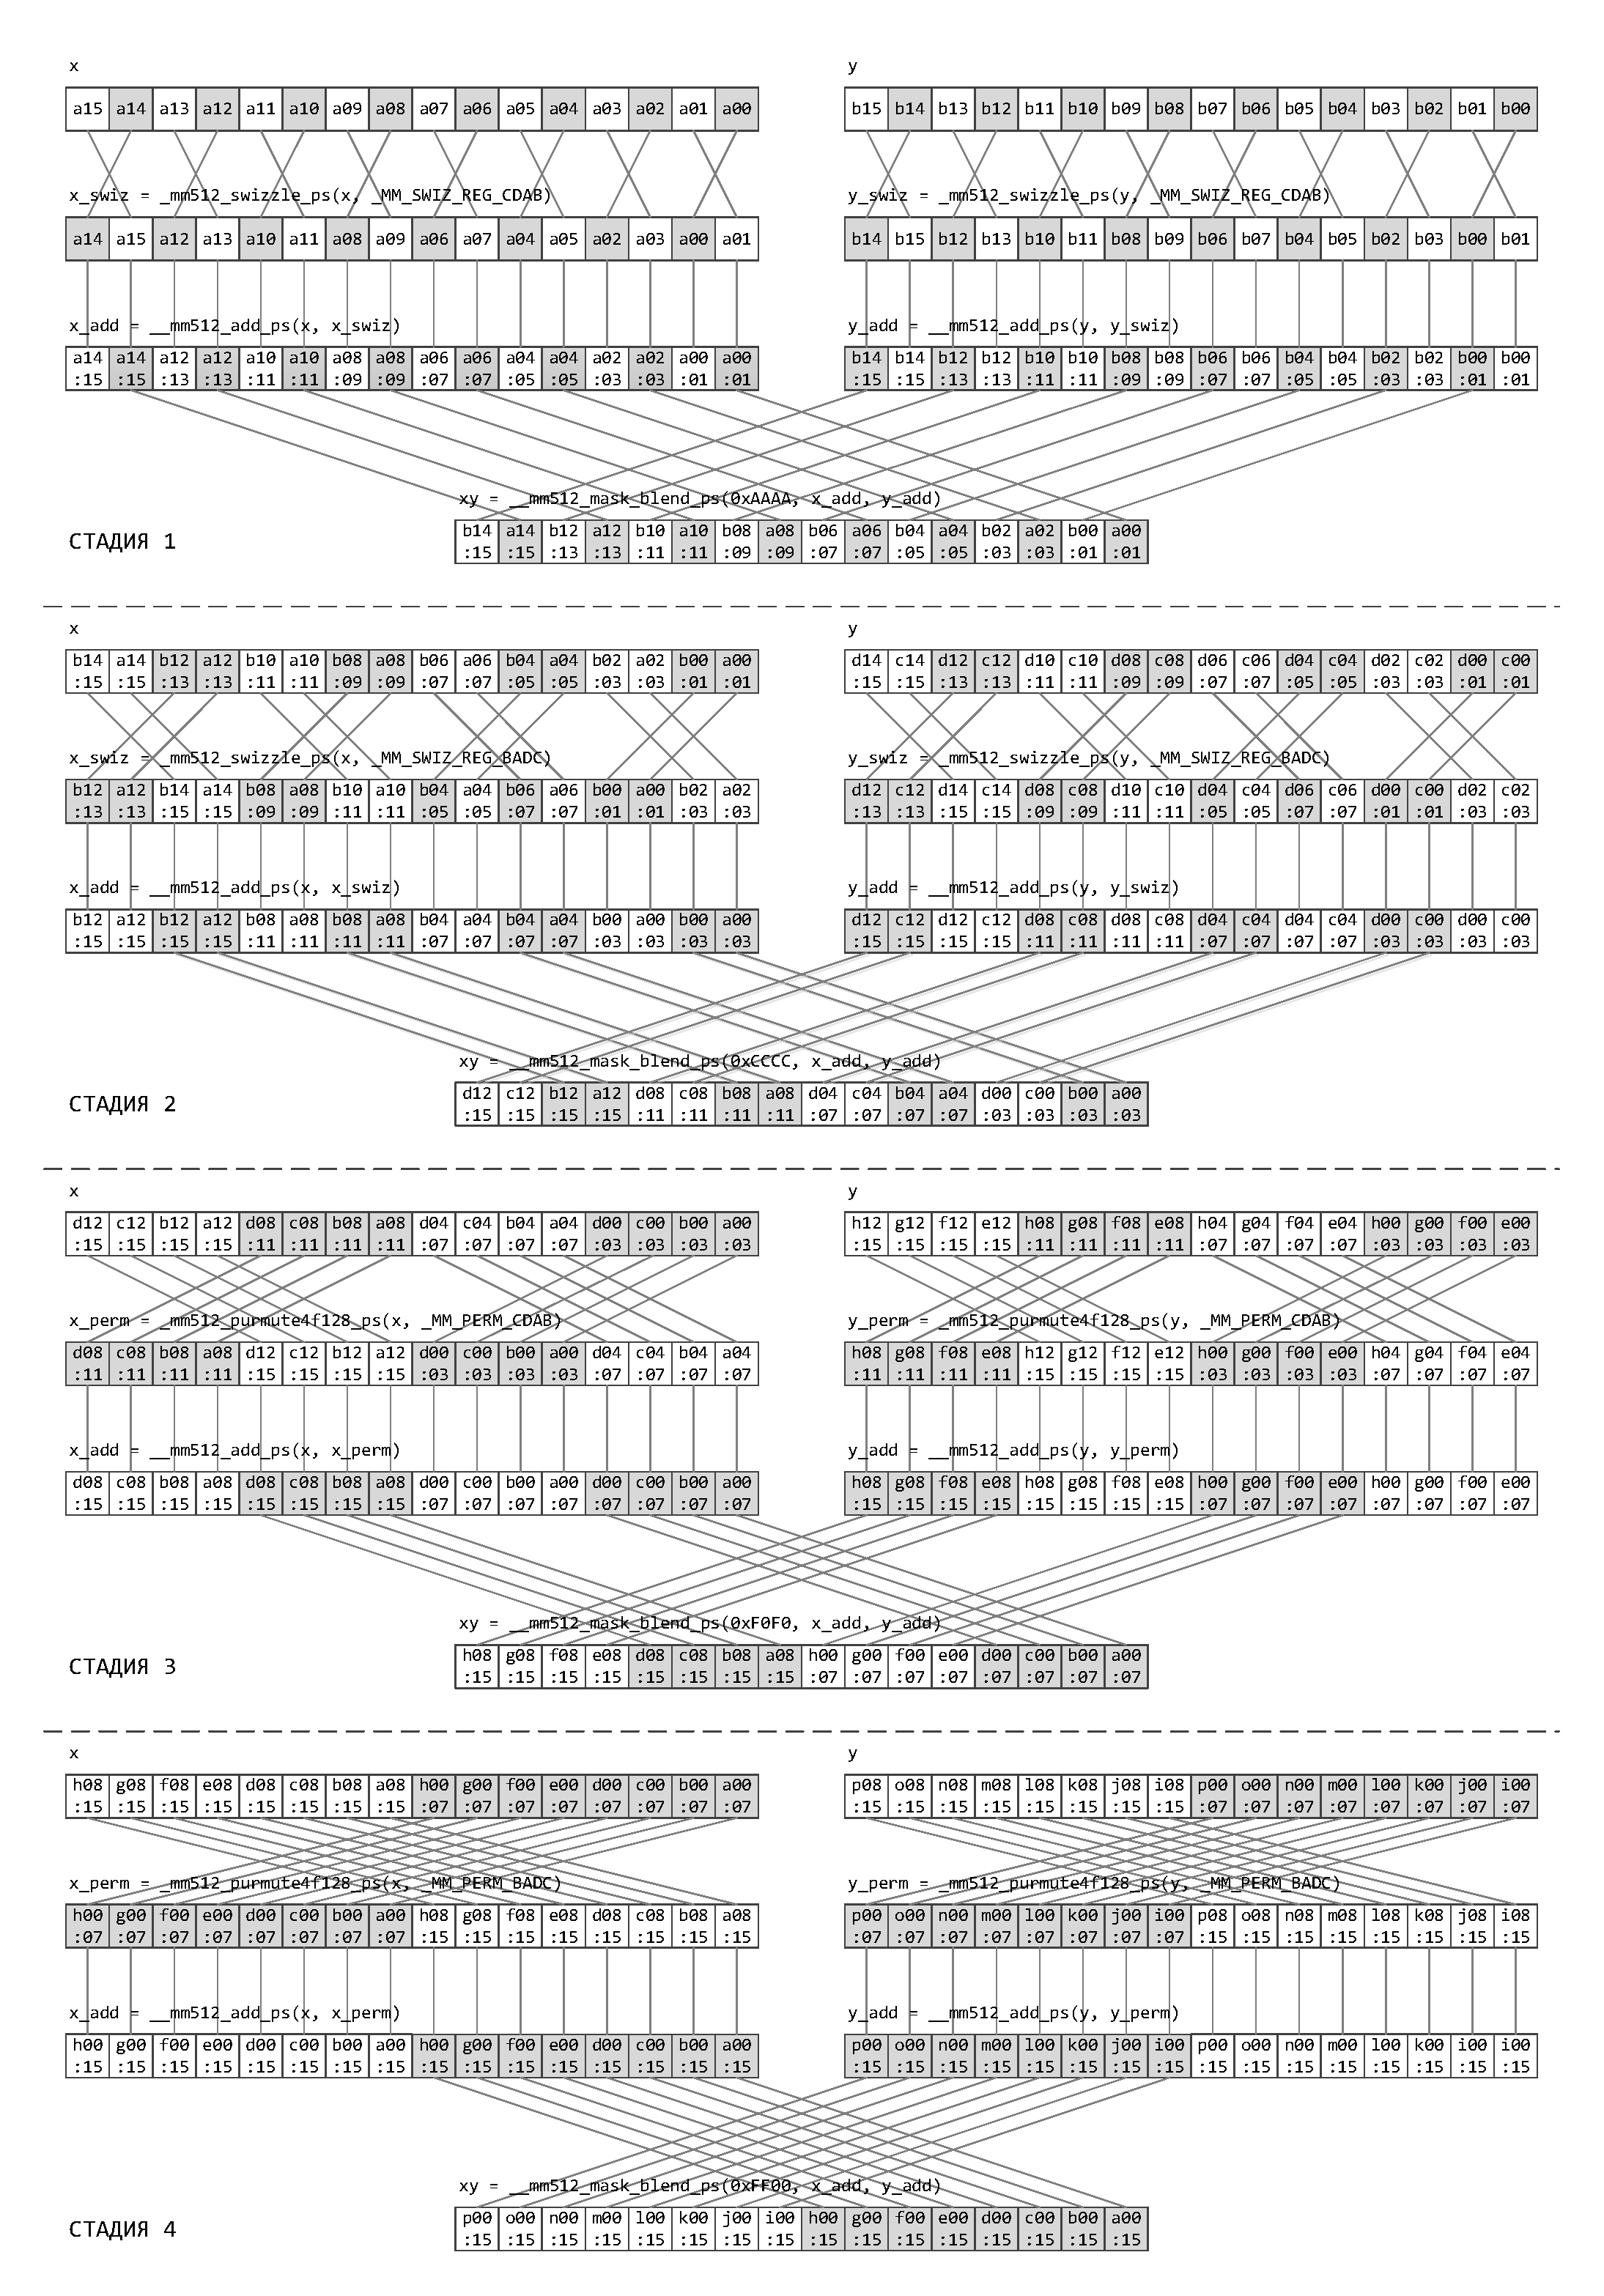
\includegraphics[width=0.67\textwidth]{./pics/text_4_small_matr/horizontal_add.pdf}
	\caption{Схема суммирования элементов zmm вектора}
	\label{fig:text_4_small_matr_horizontal_add}
\end{figure}

Набор команд AVX-512 не содержит операций горизонтального сложения элементов вектора.
Таким образом, для сложения двух элементов одного и того же вектора требуется покомпонентно сложить этот вектор со своей копией, в которой элементы переставлены нужным образом.
Это действие и выполняется на каждой обозначенной на рис. 3 фазе.
Так как всего вектор содержит 16 элементов, то минимальное количество фаз, необходымых для суммирования его элементов равно 4.
После первой фазы (после выполнения операции слияния blend) можно наблюдать вектор, содержащий суммы пар соседних элементов векторов a и b, после второй фазы вектор состоит уже из сумм четверок элементов векторов a, b, c и d, и т. д
На рис 4. представлен граф потока данных для осуществления суммирования всех элементов 16 векторов.
При этом черными квадратами обозначены операции перестановки элементов (swizzle или purmute в терминах интринсиков), черными кругами обозначены операции сложения вектора со своей пермутированной копией, а белые круги обозначают операции слияния двух векторов по маске.
Прямоугольниками с пунктирной границей очерчены фазы из рис. 3.

\begin{figure}[ht]
	\centering
		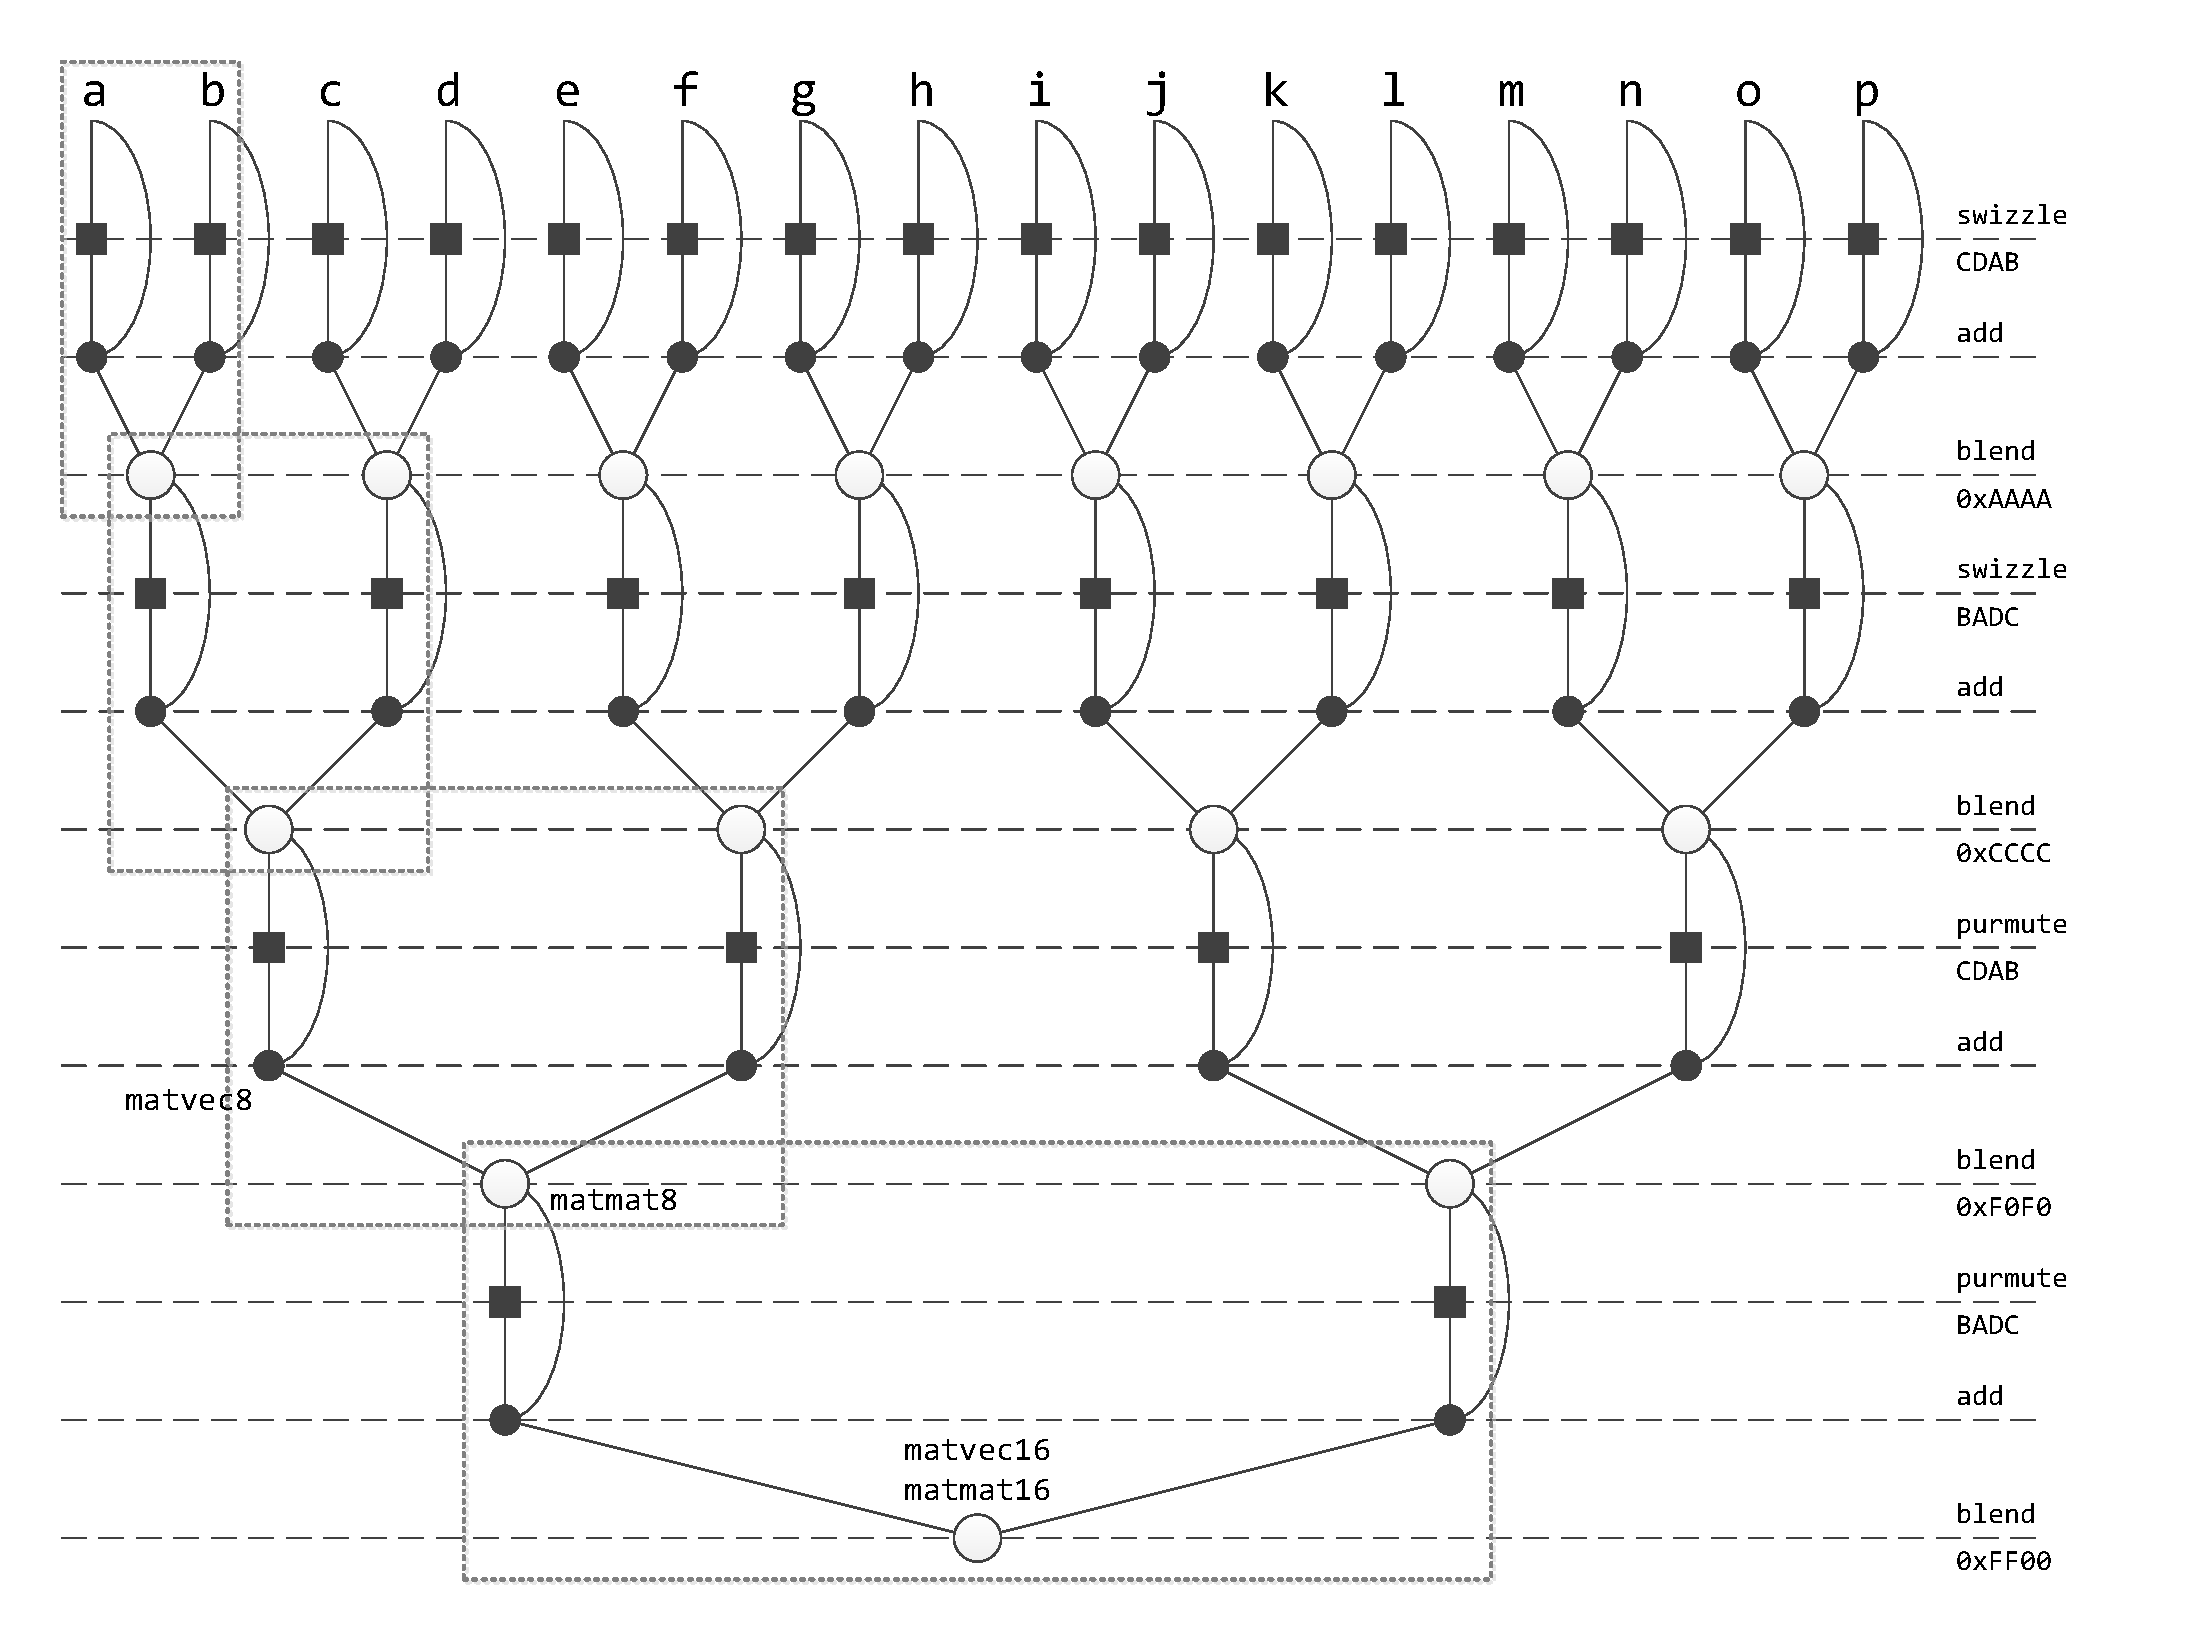
\includegraphics[width=0.8\textwidth]{./pics/text_4_small_matr/operations_tree.pdf}
	\caption{Схема суммирования элементов 16 zmm векторов}
	\label{fig:text_4_small_matr_operations_tree}
\end{figure}

Можно заметить, что граф потока данных на рис. 4 состоит из схожих блоков операций, выполняющих одни и те же действия с разными входными регистрами: пермутация двух векторов, сложение пары векторов с пермутированной копией и слияние этих двух результатов по маске (2 swizzle/permute + 2 add + 1 blend).
Причем на каждой фазе свои маски перестановок и слияний, но они постоянны для всех входных векторов.
Для удобства можно определить макросы, реализующие обозначенные фазы. На вход макрос получает пару обрабатываемых векторов, а также параметры перестановки элементов и слияния результирующей пары.
Пара макросов объясняется тем, что интринсик swizzle предназначен для перестановки элементов внутри 128-битных четвертей, а permute4f128 переставляет местами эти четверти (обе функции раскрываются в операцию perm).

\begin{lstlisting}[caption={Макрос SWIZ}, label={lst:text_4_small_matr_swiz_macro}]
#define SWIZ_2_ADD_2_BLEND_1(X, Y, SWIZ_TYPE, BLEND_MASK) \
    _mm512_mask_blend_ps(BLEND_MASK, \
                         _mm512_add_ps(X, _mm512_swizzle_ps(X, SWIZ_TYPE)), \
                         _mm512_add_ps(Y, _mm512_swizzle_ps(Y, SWIZ_TYPE)))

#define PERM_2_ADD_2_BLEND_1(X, Y, PERM_TYPE, BLEND_MASK) \
    _mm512_mask_blend_ps(BLEND_MASK, \
                         _mm512_add_ps(X, _mm512_permute4f128_ps(X, PERM_TYPE)), \
                         _mm512_add_ps(Y, _mm512_permute4f128_ps(Y, PERM_TYPE)))
\end{lstlisting}

Есть еще один похожий вариант выполнения одной фазы, реализующийся последовательностью операций 2 swizzle/permute + 2 blend + 1 add, но он оказался менее эффективным, поэтому не приводится.

Последний рассматриваемый в статье пример -- нахождение обратной матрицы.
Приведем краткое описание алгоритма Гаусса-Жордана для нахождения обратной матрицы и опишем пути оптимизации реализации соответствующей функции \texttt{invmat8\_orig}.

\subsubsection{Нахождение обратной матрицы с помощью алгоритма Гаусса-Жордана}

Последний рассматриваемый в статье пример -- нахождение обратной матрицы.
Приведем краткое описание алгоритма Гаусса-Жордана для нахождения обратной матрицы и опишем пути оптимизации реализации соответствующей функции \texttt{invmat8\_orig}.

По данному алгоритму к исходной матрице m нужно приписать справа единичную матрицу e.
Получим прямоугольную матрицу вида (a|e), размера 8x16.
Далее над этой матрицей необходимо выполнить такие преобразования строк (перестановка строк, умножение строк на постоянное число, прибавление к одной строке другой строки, умноженной на постоянное число), чтобы исходная матрица, стоящая слева, трансформировалась в единичную.
Тогда матрица, стоящая справа, из единичной трансформируется в искомую обратную матрицу.
Для достижения этого эффекта выполняется следующая последовательность действий (цикл по i от 0 до 8):

\begin{figure}[ht]
	\centering
		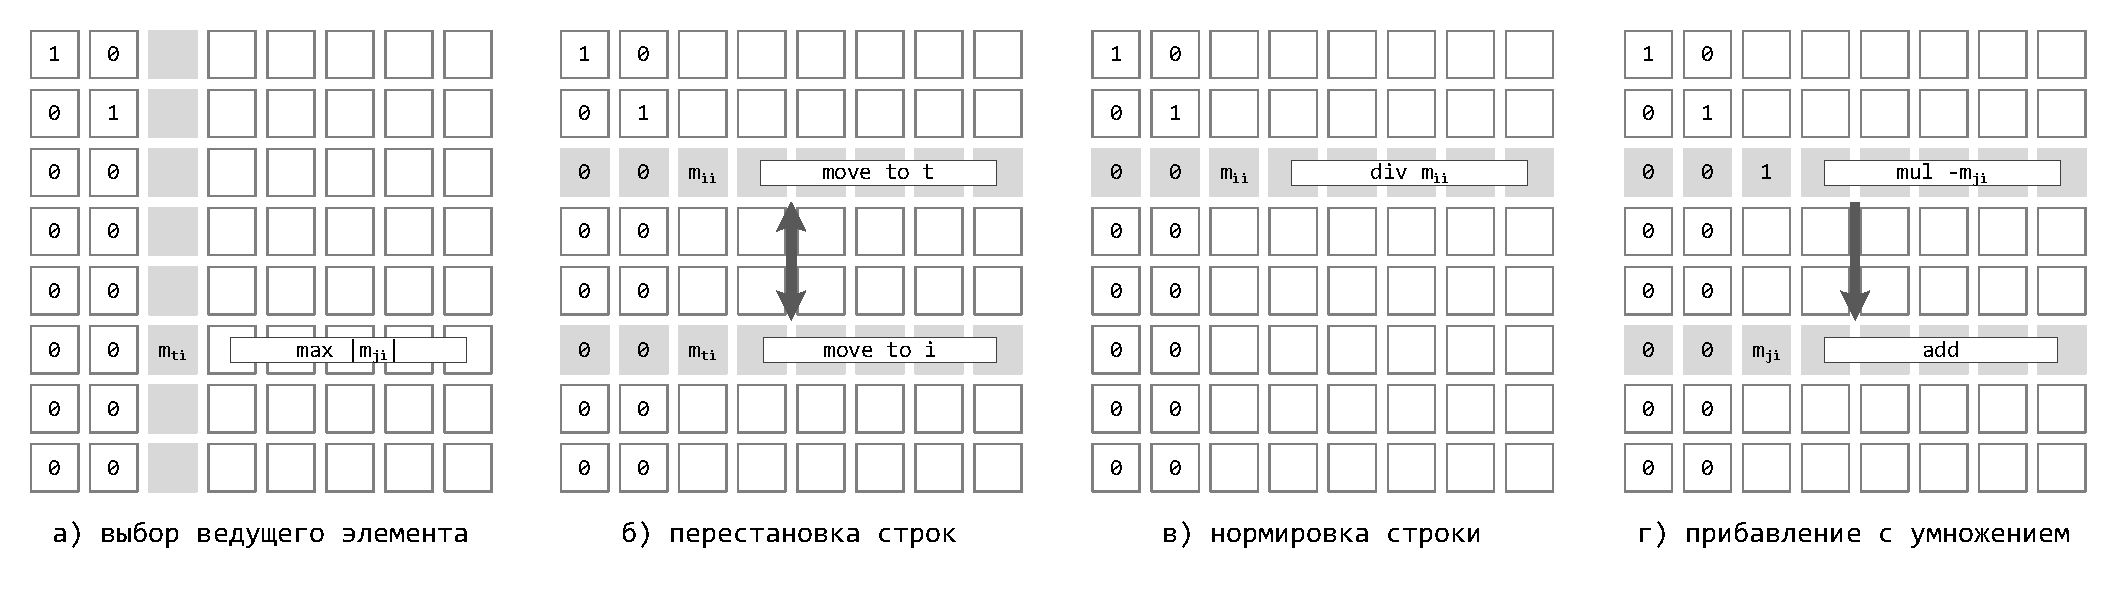
\includegraphics[width=0.8\textwidth]{./pics/text_4_small_matr/invmat8.pdf}
	\caption{Базовые действия алгоритма Гаусса-Жордана нахождения обратной матрицы}
	\label{fig:text_4_small_matr_invmat8}
\end{figure}

Поиск ведущей строки с максимальным абсолютным значением i-го элемента (рис. 5. а).
Если такое значение равно нулю, то матрица вырождена.
Это единственное место алгоритма, которое плохо поддается векторизации, к тому же содержит аварийный выход.
Данное действие занимает небольшую часть вычислений и не сказывается на производительности, поэтому ручная оптимизация в данном случае не применялась;

Перестановка ведущей строки и i-ой строки местами (рис. 5. б).
После выполнения этого действия элемент mii является максимальным по абсолютному значению элементом i-го столбца.
Действие успешно векторизуется с помощью операций пересылки zmm векторов;

Нормировка i-ой строки матрицы, то есть деление всех ее элементов на mii (рис. 5. в).
После выполнения этого действия элемент mii равен единице.
Реализуется одной операцией упакованного деления (или упакованного умножения на обратный элемент);

С помощью i-ой строки обнуление всех i-ых элементов во всех остальных строках (рис. 5. г).
Выполняется путем прибавления i-ой строки, умноженной на нужный коэффициент, к каждой строке матрицы.
Для этого действия применяются упакованные FMA операции, которые существенно ускоряют код.

Однако нужно сделать одну оговорку.
Описанные выше действия выполняются над строками матрицы размера 8x16, последовательно хранящейся в памяти.
Но на вход функции подается матрица 8x8, также хранящаяся в памяти последовательно.
Поэтому внутри функции возникают накладные действия, связанные с копированием элементов входной матрицы во временную матрицу 8x16 и обратным копированием из временной матрицы результата.
Также требуется инициализация правой части временной матрицы элементами единичной матрицы.
Все эти накладные действия реализуются с помощью операций gather/scatter.
Заметим, что при реализации \texttt{invmat16} накладные расходы не обязательны, так как нет смысла объединять две матрицы 16x16 в одну временную матрицу 16x32 (строка объединенной матрицы, содержащая 32 значения типа float, все равно не поместится в zmm регистр).

\subsubsection{Реализационная часть}

В данном разделе статьи приводятся оптимизированные фрагменты для описанных выше функций реализации операций с малоразмерными матрицами.
В реализации функции \texttt{matvec8\_opt} следует отметить загрузку двух копий вектора в zmm регистр с помощью операции gather.
Существует возможность загрузки двух копий 256-битного участка памяти в zmm регистр, однако реализована она с помощью интринсика \texttt{\_mm512\_extload\_pd} с указанием параметра \texttt{\_MM\_BROADCAST\_4X8}.
Так как формально в данном случае результатом является регистр типа \texttt{\_\_m512d}, то было решено оставить чтение через gather.
Выполнение горизонтальных операций суммирования половинок четырех zmm регистров заканчивается на операции add третьей фазы, как показано на рис. 3.

\begin{lstlisting}[caption={caption}, label={label}]
void matvec8_opt(float* __restrict m, float* __restrict v, float* __restrict r)
{
    ...
    vec = _mm512_i32gather_ps(_mm512_set_epi32(7, 6, 5, 4, 3, 2, 1, 0,
                                               7, 6, 5, 4, 3, 2, 1, 0),
                              v, _MM_SCALE_4);
    ...
    m0 = _mm512_mul_ps(_mm512_load_ps(&m[0]), vec);
    ...
    x0 = SWIZ_2_ADD_2_BLEND_1(m0, m2, _MM_SWIZ_REG_CDAB, 0xAAAA);
    x2 = SWIZ_2_ADD_2_BLEND_1(m4, m6, _MM_SWIZ_REG_CDAB, 0xAAAA);
    m0 = SWIZ_2_ADD_2_BLEND_1(x0, x2, _MM_SWIZ_REG_BADC, 0xCCCC);
    x0 = _mm512_add_ps(m0, _mm512_permute4f128_ps(m0, _MM_PERM_CDAB));
    ...
    _mm512_mask_i32scatter_ps(r, 0xF0F,
                              _mm512_set_epi32(0, 0, 0, 0, 7, 5, 3, 1,
                                               0, 0, 0, 0, 6, 4, 2, 0),
                              x0, _MM_SCALE_4);
}
\end{lstlisting}

Перемножение двух матриц изначально реализуется гнездом из трех вложенных циклов.
Два внешних цикла относятся к проходу по строкам одной из перемножаемых матриц и столбцам другой (за одну итерацию обрабатывается по две строки и по два столбца соответственно).
Внутренний цикл считает скалярное произведение соответствующей строки и столбца.
Так как строки матрицы занимают в памяти последовательные участки, то чтение двух соседних строк выполняется обычной функцией \texttt{\_mm512\_load\_ps}.
Загрузку же двух соседних столбцов следует выполнять с использованием gather и заданными смещениями всех элементов.
По этой причине в реализации была выполнена перестановка двух внешних циклов, чтобы чтение с помощью gather выполнялось во внешнем цикле, так как данная операция более медленная, чем чтение последовательного участка памяти.
Далее выполняется полная раскрутка ставшего теперь уже внутренним цикла, проходящего по строкам матрицы a.
Выполнение горизонтальных операций суммирования половинок 8 регистров zmm заканчивается на операции blend третьей фазы из рис. 3.
Полученные 16 элементов результирующей матрицы записываются в память с использованием scatter с указанием смещений.

\begin{lstlisting}[caption={caption}, label={label}]
void matmat8_opt(float* __restrict a, float* __restrict b, float* __restrict r)
{
	...
    ind = _mm512_set_epi32(7 * V8 + 1, 6 * V8 + 1, 5 * V8 + 1, 4 * V8 + 1,
                           3 * V8 + 1, 2 * V8 + 1,     V8 + 1,          1,
                               7 * V8,     6 * V8,     5 * V8,     4 * V8,
                               3 * V8,     2 * V8,         V8,          0);

    for (int j = 0; j < V8; j += 2)
    {
        ...
        bj = _mm512_i32gather_ps(ind, &b[j], _MM_SCALE_4);
        bj2 = _mm512_permute4f128_ps(bj, _MM_PERM_BADC);
        ...
        a0 = _mm512_load_ps(&a[ii0]);
        m0 = _mm512_mul_ps(a0, bj);
        m1 = _mm512_mul_ps(a0, bj2);

        ...
        x0 = SWIZ_2_ADD_2_BLEND_1(m0, m1, _MM_SWIZ_REG_CDAB, 0xAAAA);
        x1 = SWIZ_2_ADD_2_BLEND_1(m2, m3, _MM_SWIZ_REG_CDAB, 0xAAAA);
        x2 = SWIZ_2_ADD_2_BLEND_1(m4, m5, _MM_SWIZ_REG_CDAB, 0xAAAA);
        x3 = SWIZ_2_ADD_2_BLEND_1(m6, m7, _MM_SWIZ_REG_CDAB, 0xAAAA);
        m0 = SWIZ_2_ADD_2_BLEND_1(x0, x1, _MM_SWIZ_REG_BADC, 0xCCCC);
        m1 = SWIZ_2_ADD_2_BLEND_1(x2, x3, _MM_SWIZ_REG_BADC, 0xCCCC);
        x0 = PERM_2_ADD_2_BLEND_1(m0, m1, _MM_PERM_CDAB, 0xF0F0);
        ...
        ind1 = _mm512_set_epi32(ii3 + V8 + j, ii3 + V8 + j + 1,
                                ii2 + V8 + j, ii2 + V8 + j + 1,
                                ii1 + V8 + j, ii1 + V8 + j + 1,
                                ii0 + V8 + j, ii0 + V8 + j + 1,
                                 ii3 + j + 1,          ii3 + j,
                                 ii2 + j + 1,          ii2 + j,
                                 ii1 + j + 1,          ii1 + j,
                                 ii0 + j + 1,          ii0 + j),
        _mm512_i32scatter_ps(r, ind1, x0, _MM_SCALE_4);
    }
\end{lstlisting}

Реализация функции \texttt{invmat8\_opt} начинается с формирования временной матрицы размера 8x16, левой частью которой становится входная матрица, а в правой считается результат.
Входная матрица копируется во временную с помощью четырех пар операций load - scatter, одновременно обнуляется правая часть матрицы. 
После этого для завершения инициализации единичной матрицы в правой части временной матрицы в нее с помощью операции scatter записывается вектор, состоящий из единиц, с указанием расстояния между записями V16 + 1.
После инициализации временной матрицы выполняется тело алгоритма Гаусса-Жордана нахождения обратной матрицы.
Действие по нахождению ведущей строки не подвергалось векторизации. Прежде всего там присутствует горизонтальная операция, связанная с нахождением максимального по модулю элемента некоторого столбца временной матрицы.
Кроме того, во время поиска ведущей строки возможен аварийный выход из функции, поэтому попытки оптимизации данного фрагмента нецелесообразны.
Три остальные действия реализуются без каких бы то ни было особенностей с помощью применения пересылок и покомпонентных операций сложения, умножения и комбинированных FMA операций.

\begin{lstlisting}[caption={caption},label={label}]
int invmat8_opt(float* __restrict m, float* __restrict r)
{
    ........................................
    __m512i ind = _mm512_set_epi32(V16 + 7, V16 + 6, V16 + 5, V16 + 4,
                                   V16 + 3, V16 + 2, V16 + 1,     V16,
                                         7,       6,       5,       4,
                                         3,       2,       1,       0);

    for (int i = 0; i < V8; i += 2)
    {
        _mm512_i32scatter_ps(&t[i * V16], ind, _mm512_load_ps(&m[i * V8]), _MM_SCALE_4);
        _mm512_i32scatter_ps(&t[i * V16 + V8], ind, _mm512_setzero_ps(), _MM_SCALE_4);
    }

    __m512i ind1 = _mm512_set_epi32(0, 0, 0, 0, 0, 0, 0, 0,
                                    7 * V16 + 7, 6 * V16 + 6,
                                    5 * V16 + 5, 4 * V16 + 4,
                                    3 * V16 + 3, 2 * V16 + 2,
                                        V16 + 1,           0);
    _mm512_mask_i32scatter_ps(&t[V8], 0xFF, ind1, _mm512_set1_ps(1.0), _MM_SCALE_4);

    for (int i = 0; i < V8; i++)
    {
        ...
        if (lead_i != i)
        {
            int ll = lead_i * V16;

            vi = _mm512_load_ps(&t[ii]);
            vl = _mm512_load_ps(&t[ll]);
            _mm512_store_ps(&t[ll], vi);
            _mm512_store_ps(&t[ii], vl);
        }
        ...
        vd = _mm512_set1_ps(1.0 / t[ii + i]);
        vi = _mm512_load_ps(&t[ii]);
        vi = _mm512_mul_ps(vi, vd);
        _mm512_store_ps(&t[ii], vi);
        ...
        for (int j = 0; j < V8; j++)
        {
            int jj = j * V16;

            if (j != i)
            {
                vd = _mm512_set1_ps(-t[jj + i]);
                vj = _mm512_load_ps(&t[jj]);
                vi = _mm512_load_ps(&t[ii]);
                vj = _mm512_fmadd_ps(vi, vd, vj);
                _mm512_store_ps(&t[jj], vj);
            }
        }
    }

    ...
    for (int i = 0; i < V8; i += 2)
    {
        vi = _mm512_i32gather_ps(ind, &t[i * V16 + V8], _MM_SCALE_4);
        _mm512_store_ps(&r[i * V8], vi);
    }
}
\end{lstlisting}

После завершения работы алгоритма Гаусса-Жордана результат из временной матрицы перемещается в область памяти результата с помощью пар операций gather - store.

Реализация функций по работе с матрицами 16x16 не приводится, так как данные функции имплементируются аналогично, только код получается более громоздкий.
Выполнение горизонтальных операций сложения для matvec16 и matmat16 охватывает все четыре фазы из рис. 3, логика же вычислений более примитивна, так как не требуется объединения итераций при обходе матриц - одна строка матрицы в точности заполняет zmm регистр.

\subsubsection{Экспериментальная часть}

Реализованные в рамках данной работы оптимизированные с помощью инструкций AVX-512 функции для работы с малоразмерными матрицами были опробованы на процессоре Intel Xeon Phi KNL 7290.
Данные процессоры входят в состав суперкомпьютера МВС-10П, находящегося в МСЦ РАН.
Был выполнен анализ эффективности примененных оптимизаций.
Для этого рассматривались два варианта исполняемого кода. В первом варианте функции были реализованы без использования интринсиков, компилировались с использованием компилятора icc с указанием -xmic-avx512 и уровнем оптимизации -O3.
Во втором варианте использовались те же опции компиляции, однако функции были оптимизированы вручную, как это было описано в предыдущих разделах.
В обоих вариантах был запрещен инлайн рассматриваемых функций в место вызова.
Рассматривались функции умножения матрицы на вектор, перемножения двух матриц и нахождения обратной матрицы.
Размеры матриц рассматривались в двух вариантах: 8x8 и 16x16.
Всего было рассмотрено 6 функций: matvec8, matvec16, matmat8, matmat16, invmat8, invmat16. 

На рис. 6 приведены данные о сокращении времени работы оптимизированных функций, реализующих операции над малоразмерными матрицами.
За 100\% принято время исполнения функций, реализованных без использования интринсиков.

\begin{figure}[ht]
	\centering
		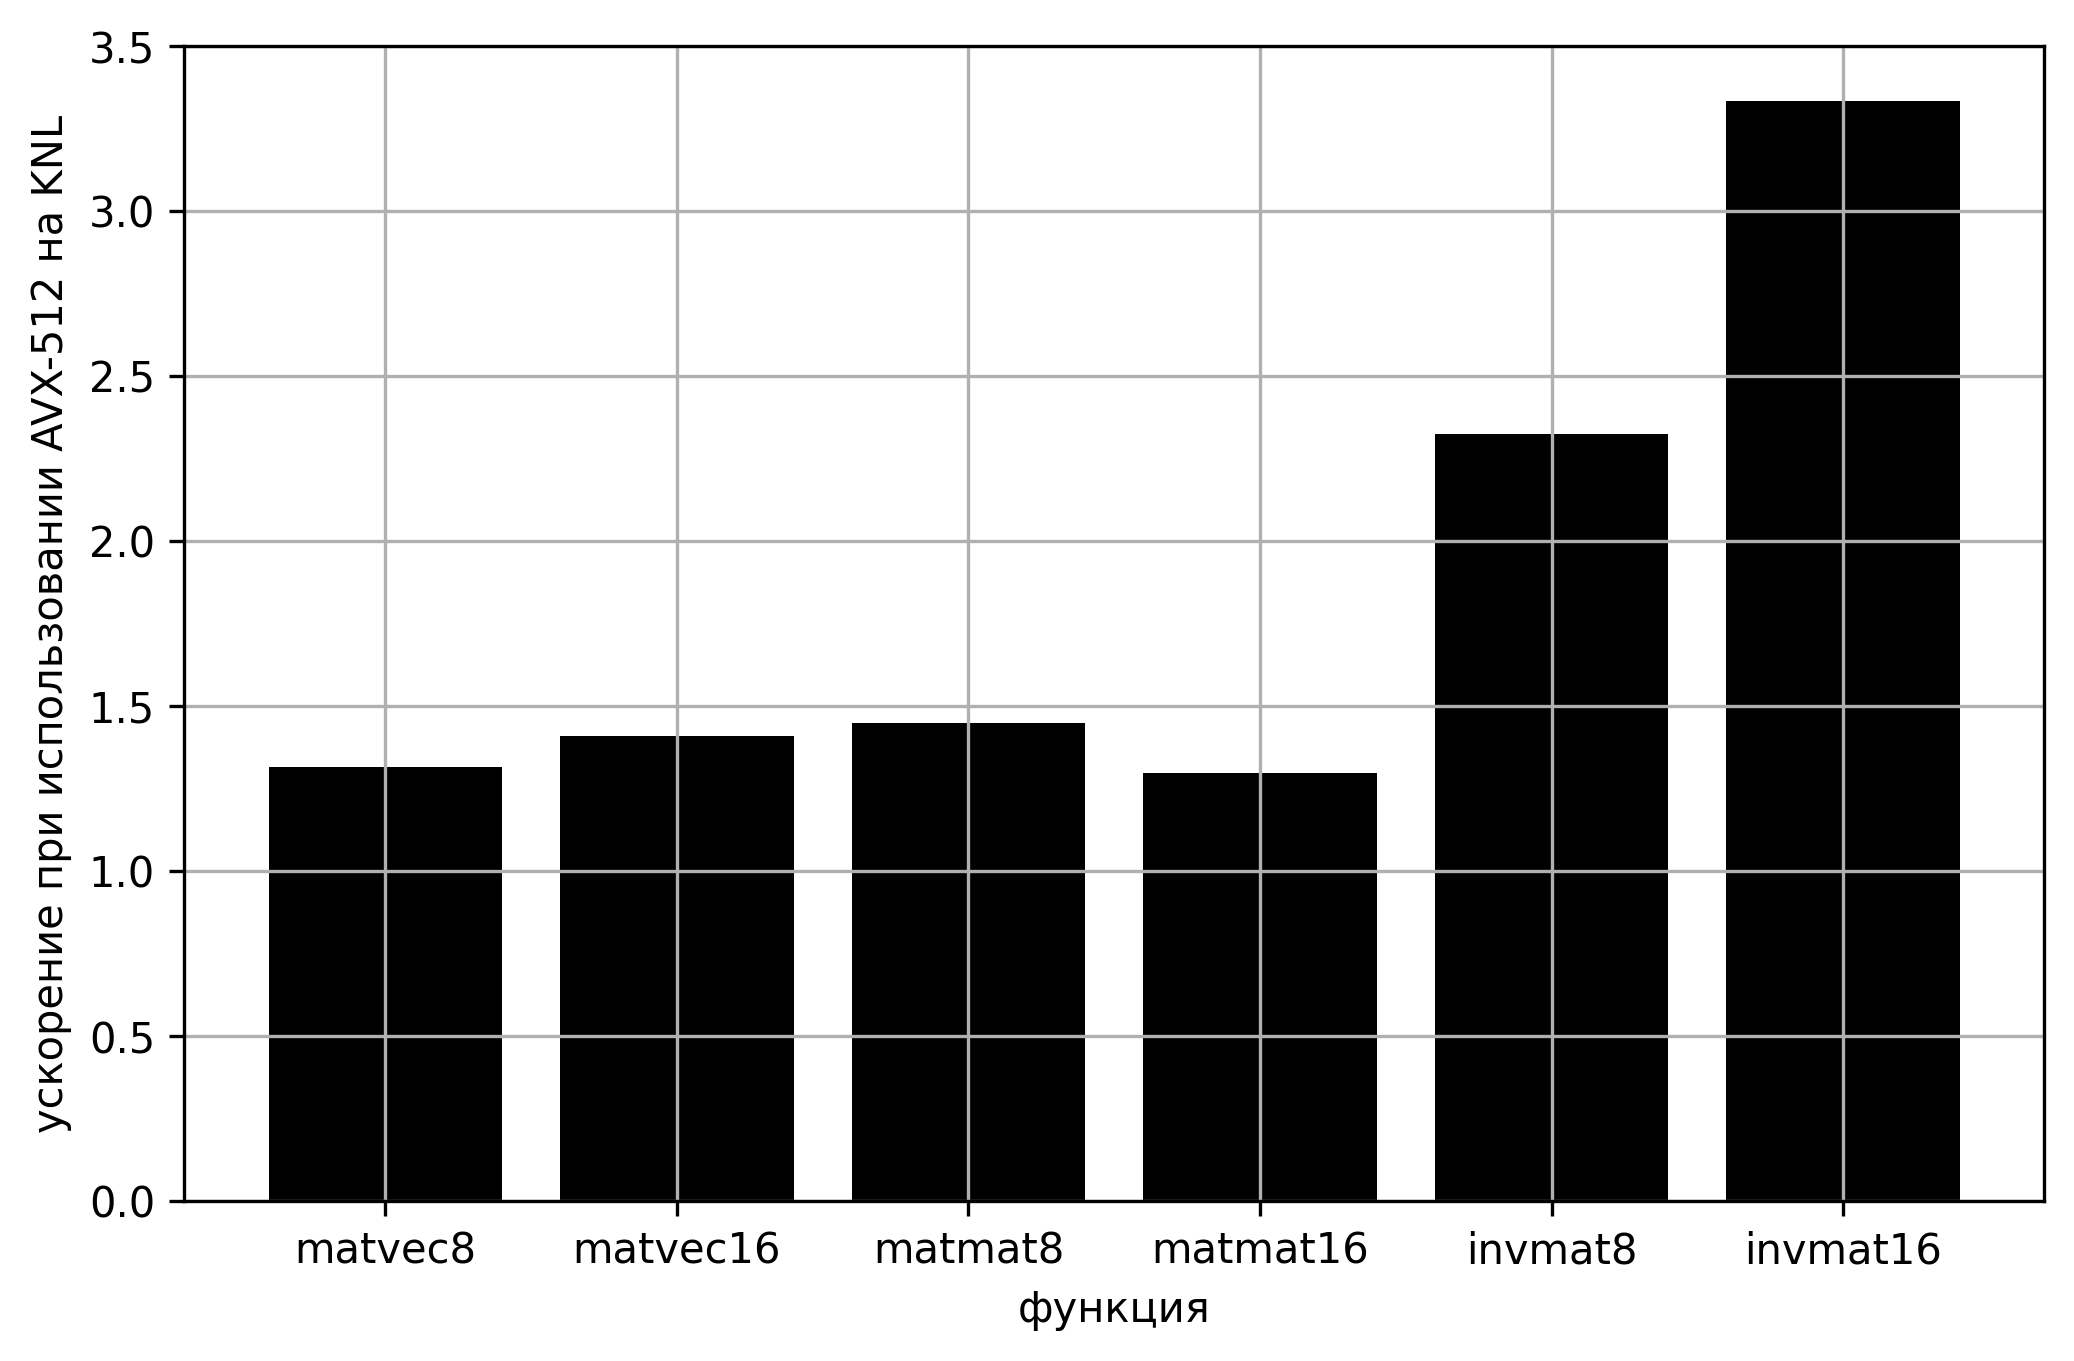
\includegraphics[width=1.00\textwidth]{./pics/text_4_small_matr/res.png}
	\caption{Сокращение времени работы оптимизированных версий операций над малоразмерными матрицами}
	\label{fig:text_4_small_matr_res}
\end{figure}

Темным цветом на гистограмме отмечено время исполнения вариантов функций, реализованных с явным использованием 512-битных векторных операций.
Наибольшее ускорение продемонстрировали функции нахождения обратной матрицы, так как алгоритм нахождения обратной матрицы естественным образом формулируется в терминах работы со строками объединенной матрицы, что находит свое отражение в 512-битных векторных операциях.
При этом функция invmat16 ускорилась больше, чем invmat8, потому что, в отличие от последней, она не содержит накладных действий, связанных с копированием входной матрицы во временную матрицу, а затем чтением результата из временной матрицы. Функции matvec и matmat демонстрируют умеренное ускорение.
Причиной тому служит наличие горизонтальных операций сложения, которые порождают длинный критический путь исполнения внутри функции.
Объединение горизонтальных операций позволяет сгладить этот эффект, однако для дальнейшего ускорения требуется реализация объединенных функций, выполняющих одновременно сразу несколько операций или применяющих одну операцию к более широкому набору данных (например, функция перемножение двух пар матриц).
